\documentclass[11pt, a4paper]{report}
\usepackage[utf8]{inputenc}

\usepackage{listings}
\usepackage[framed,numbered,autolinebreaks,useliterate]{mcode}

\usepackage[margin=1in]{geometry}
\usepackage{graphicx}
\usepackage{amsmath}
\usepackage{amsfonts}
\usepackage{float}
\graphicspath{ {images/} }
\setlength\parindent{0pt}


\newcommand{\p}{\partial}
\newcommand{\mth}[1]{
  \begin{align*}
    #1
  \end{align*}
}



\begin{document}

\begin{center}
  \Huge Floppy Drive Orchestra \\
  \huge University of Colorado Boulder \\
  \Large Independent Study\\
  
  \vspace{6in}
    \huge Jeffery Lim \\
    \huge Jeffery.Lim@colorado.edu\\
    \Large Under supervision of Dr. Shalom Ruben \\~\\~\\
\end{center}
\pagebreak

\tableofcontents

\chapter{Introduction}
\chapter{Floppy Drive Characteristics}

In order to properly proceed to develop a floppy drive orchestra, a single floppy drive must be understood in order to understand the capabilities and restrictions that the floppy drives presents. 


\section{Floppy Pinout}

The floppy pinout is shown in Figure \ref{fig:pinOut}. The bottom row, or the odd valued pins, are all grounded, where the top pins, or the even valued pins, are live. The actual names of the active pins are shown in Figure \ref{fig:pinNames}
\begin{figure}[H]
\hspace*{-2cm}    
    \centering
    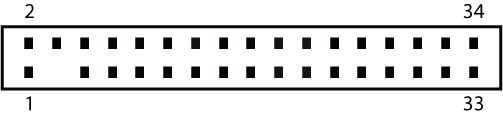
\includegraphics[width=.75\textwidth]{floppy_pinout.jpg}
    \caption{Floppy Drive Pinout}
    \label{fig:pinOut}
\end{figure}

\begin{figure}[H]
\hspace*{-2cm}    
    \centering
    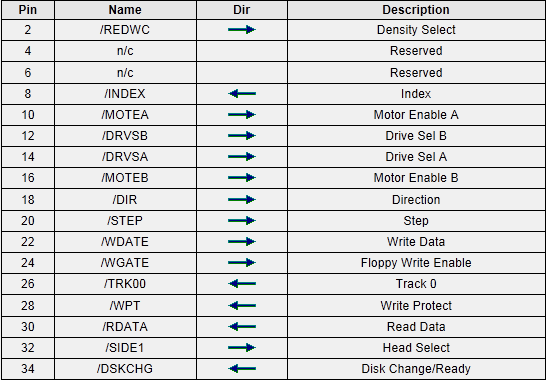
\includegraphics[width=.75\textwidth]{pinNames.png}
    \caption{Floppy Drive Pin Names}
    \label{fig:pinNames}
\end{figure}

The only necessary pins are pin number 12 or 14, 18, and 20. Pins 12 and 14 are the drive select B and A. These are the drive enable pins. Some drives are B drives and others are A, so in order to test them, either one of them will need to be sleected.\\

Pin 18 is a direction pin. The direction is what determins the direction of the motor drive. When the pin is grounded, the drive heads away from the pins, and when the pin is high, the drive returns. \\

Pin 20 is a step pin. This pin drives the stepper motor, so every time the pin goes high, the stepper motor will go forward one tick. \\

\section{Stepper Motor Movement}

The floppy drive motor head has a physical limit to how far it can go. To determine this value, a 1 Hz square wave is sent through to the floppy drive's direction pin (pin 18). The number of ticks is manually recorded, and the step pin is inverted, to count back. \\

The total number of ticks a drive can go is 80, meaning the step pin (pin 20) needs to be toggled 80 times before the drive reaches the limit. Depending on the floppy drive, the motor will either continue to try and go forward, and others will not move. \\

\section{Stepper Motor Bandwidth}

Since the music will be played through the motor head, the bandwidth of the stepper motor will be a large limiting factor. For the test, a square wave from a waveform generator is connected to the step pin (pin 20), and the direction pin is connected to ground and disconnected in order to allow the motor head to switch direction. \\

The waveform generator is swepted from 1 Hz up until the motor head is no longer moving. The drive was able to handle up to 400 Hz, but afterwords, it was no longer consistent in terms of the speed of the drive. \\

This limit considerably restricts what the drive can play, and higher notes will need to be address. 


\section{Power}

The floppy drive takes a mini Molex cable as seen in Figure \ref{fig:miniMolex}. A mini Molex cable has a 5V line as well as 12V. Modern floppy drives used to use the 12V line for the drive motor, however, more modern floppy drives only use the 5V to drive the entire drive. \\

The power consumption of the drive when idling is an average of 50 mA and when the motor is active, it pulls 400 mA. \\


\chapter{Wiring Diagram}

Because the floppy drive only requires 5V and 400 mA each, there are two approaches in order to supply the power. A 5V power source with enough current to support all the drives is sufficient to power the system.
\section{Power}

\begin{figure}[H]
\hspace*{-2cm}    
    \centering
    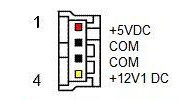
\includegraphics[width=.3\textwidth]{miniMolex.jpg}
    \caption{Floppy Drive Power Pinout}
    \label{fig:miniMolex}
\end{figure}

For each floppy drive added to the system, the total power draw increases by 400 mA, so for 4 floppy drives, the total power consumption from the floppy drive system would be around 1600 mA, or 1.6 A. 
  
\section{Arduino Wiring}


\chapter{MIDI Files}

  MIDI, or Musical Instrument Digital Interface, is a standard that has its own protocols, interface, and connectors. It allows a single file to contain multiple tracks for several instruments in its own channel. This allows a MIDI file to play several instruments at once, up to a maximum of 16 instruments. This advantage of the MIDI file allows multiple floppy drives to be played at once, like how a MIDI file would send data to several instruments. 

\section{MIDI Notes}

The MIDI interface has notes that are mapped to specific piano keys at their respected frequencies. 
\begin{figure}[H]
\hspace*{-2cm}    
    \centering
    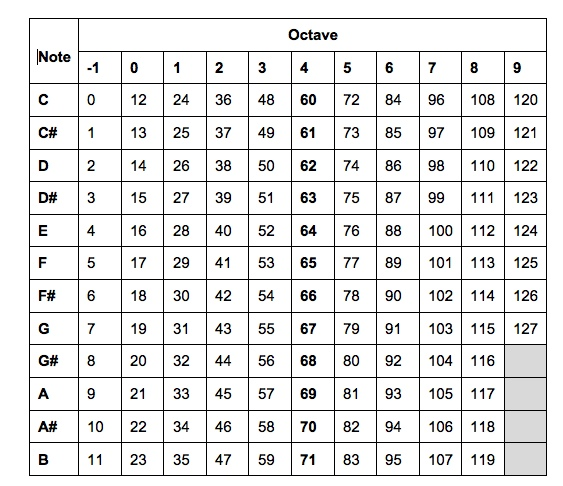
\includegraphics[width=.75\textwidth]{midi_notechart.jpg}
    \caption{MIDI Note Number to Key}
\end{figure}

\section{MIDI Messages}


\begin{center}
 \begin{tabular}{||c | c | c | c | c||} 
 \hline
  \multicolumn{5}{|c|}{MIDI Message} \\ 
 \hline\hline
  \multicolumn{3}{|c|}{Status}  & Data & Data \\
 \hline
  \multicolumn{2}{|c|} {Command (4 bits)} & Channel(4 bits)  & Note (8 bits) & Velocity (8 bits) \\
 \hline
  Note On & 1001 & nnnn  & 0xxxxxxx & 0vvvvvvv \\
 \hline  
  Note Off  & 1000 & nnnn  & 0xxxxxxx & 0vvvvvvv \\
 \hline
\end{tabular}
\end{center}

\chapter{Software}
\section{MIDI Player}
\section{MIDI to Serial Driver}
\section{Arduino}

\chapter{Arduino}
\lstinputlisting[language=C, firstline=37, lastline=45]{../src/floppy/floppy.ino}


\end{document}
